\thispagestyle{empty}
\definecolor{my_color}{RGB}{0,0,255}
\begin{center} 
	\begin{tikzpicture}[remember picture, overlay] 
		\node[anchor=north west] at (current page.north west) [xshift=1cm,yshift=-1cm] { 
			\begin{tikzpicture} 
				\draw[color=my_color, line width=3pt] (0,0) rectangle (18.8,27.6); 
				\draw[color=my_color, line width=1pt] (0.1,0.1) rectangle (18.7,27.5); 
			\end{tikzpicture} 
		}; 
		
		\node[anchor=north] at (current page.north)[yshift=-3.5cm] { 
			\includegraphics[width=0.27\textwidth,keepaspectratio]{Images/logo_issea.png} 
		}; 
		\node[anchor=north] at (current page.north)[yshift=-1.4cm] { 			
			
\begin{tikzpicture}	
				\draw[line width=2.5pt, color=my_color ] ((2,0) -- (19,0); % draws a thick line from (0,0) to (5,5) 
			\end{tikzpicture} 
		};
		
		\node[anchor=north] at (current page.north)[yshift=-2cm] { 
			\fontsize{13}{13}\selectfont COMMUNAUTÉ ÉCONOMIQUE ET MONÉTAIRE DE L’AFRIQUE 
		}; 
		\node[anchor=north] at (current page.north)[yshift=-2.5cm] { 
			\fontsize{14}{13}\selectfont (CEMAC)
		}; 
		
		\node[anchor=north] at (current page.north)[yshift=-7.5cm] { 
			\fontsize{14}{13}\selectfont	Institut Sous-régional de Statistique et 	d’Économie Appliquée (ISSEA)
		}; 
		\node[anchor=north] at (current page.north)[yshift=-8.5cm] { 
			\fontsize{14}{13}\selectfont	Organisation Internationale
		}; 
		\node[anchor=north] at (current page.north)[yshift=-9.5cm] { 
			\fontsize{14}{13}\selectfont	B.P : 294 Yaoundé
		}; 
		\node[anchor=north] at (current page.north)[yshift=-10.5cm] { 
			\fontsize{14}{13}\selectfont	www.issea-cemac.org
		}; 
		
		\node[anchor=north] at (current page.north)[yshift=-11cm] { 
			
\begin{tikzpicture}
				\draw[line width=1.3pt , color=my_color] (0,0) -- (10,0); % draws a thick line from (0,0) to (5,5) 
			\end{tikzpicture} 
		}; 
		\node[anchor=north] at (current page.north)[yshift=-11.8cm] { 
			{\shadowoffset{1.2pt}
				\setmainfont{Moving skate}
				\shadowtext{\fontsize{35}{13}\selectfont\contour{black}{\textcolor{white}{\textbf{Projet de Big Data }}}} }
				
		}; 
		
		\node[anchor=north] at (current page.north)[yshift=-13.05cm] { 
			
\begin{tikzpicture}
				\draw[line width=2.5pt , color=my_color] (0,0) -- (16,0); % draws a thick line from (0,0) to (5,5) 
				\draw[line width=0.5pt, color=my_color ] (0.5,-0.1) -- (15.5,-0.1); % draws a thick line from (0,0) to (5,5) 
			\end{tikzpicture} 
		}; 
		
		\node[anchor=north] at (current page.north) [yshift=-13.2cm] { 
			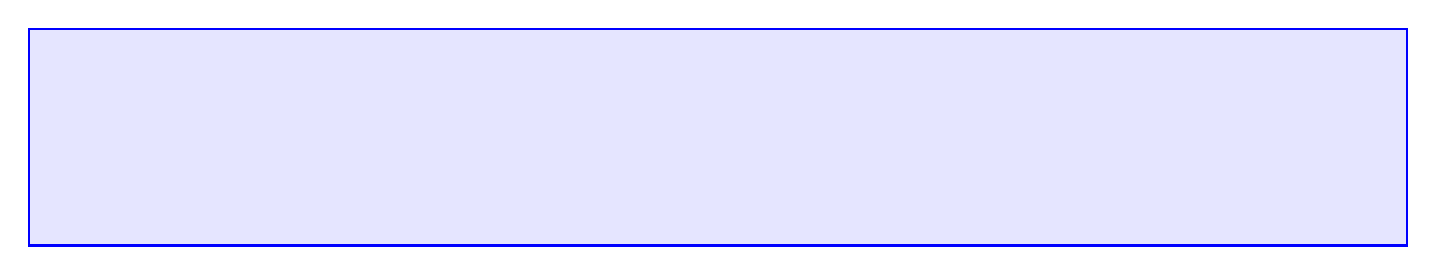
\begin{tikzpicture} 
				\draw[color=my_color, line width=1pt, fill=my_color!10] (0,0) rectangle (17.5,2.75) ; 
			\end{tikzpicture} 
		}; 				
		
		\node[anchor=north] at (current page.north)[yshift=-13.8cm,xshift=0.1cm] { 
			{\shadowoffset{1.2pt}%\setmainfont{Centaur}
				\shadowtext{\fontsize{20}{11}\selectfont\contour{black}{\textcolor{my_color}{\textbf{ANALYSE DES DONNEES LOG DU  SERVEUR  }}}} }
		}; 
		\node[anchor=north] at (current page.north)[yshift=-15cm,xshift=0.1cm] { 
			{\shadowoffset{1.2pt}%\setmainfont{Centaur}
				\shadowtext{\fontsize{20}{13}\selectfont\contour{black}{\textcolor{my_color}{\textbf{ DNS  PUBLIC DE GOOGLE VIA PYSPARK.}}}} }
		}; 
		
		
		\node[anchor=north] at (current page.north)[yshift=-15.9cm] { 			
			\begin{tikzpicture}	
				\node at (-0.1,0.2){\pgfornament[color=my_color , width=1cm ]{2}};
				\draw[line width=2.5pt, color=my_color ] ((0.6,0) -- (15,0); % draws a thick line from (0,0) to (5,5) 
				\draw[line width=0.5pt , color=my_color]((0.8,0.1) -- (14.6,0.1); % draws a thick line from (0,0) to (5,5) 
				\node[rotate=0] at (15.6,0.20){\pgfornament[color=my_color , width=1cm ,symmetry=v ]{2}};
			\end{tikzpicture} 
		};
		
\node[anchor=north] at (current page.north)[yshift=-16.7cm,xshift=-0.3cm] { 
	\begin{minipage}{1\textwidth}
		\fontsize{14}{8}\selectfont
		\begin{center}\hspace{1cm}\textbf{Rédigé par :}\end{center}
		\vspace{0.3cm}
		\begin{minipage}{0.48\textwidth}
			\begin{flushright}BESSALA Junior Serges Edouard\end{flushright}
			\begin{flushright}DAH Fongnéma\end{flushright}
			\begin{flushright}KALEFACK NGUEPI Sergeo\end{flushright}
			\begin{flushright}KEOUL Maab Mara\end{flushright}
			\begin{flushright}MAHAMAT NGAGUEDI Eric\end{flushright}
		\end{minipage}%
		 \hspace{0.7cm} 
		\begin{minipage}{0.58\textwidth}
			\begin{flushleft}MOUSSAVOU MOUSSAVOU Lloyd A. \end{flushleft}
			\begin{flushleft}NDOKO SOUAMOUNOU Geddy S. \end{flushleft}	
			\begin{flushleft}TAKOUGOUM Steeve Rodrigue \end{flushleft}
			\begin{flushleft}TAMIBE EZECHIEL Pallaye \end{flushleft}
		\end{minipage}
		\vspace{0.2cm}
		\begin{center}
			\fontsize{14}{8}\selectfont Élèves Ingénieurs Statisticiens Économistes, ISE 2
		\end{center}\vspace{-6mm}
\begin{center}
\fontsize{11}{8}\selectfont https://github.com/Githubsssssssssssssssssssssss/Big\_Data

\end{center}
\end{minipage}	
};

		
		\node[anchor=north] at (current page.north)[yshift=-24.2cm] { %\fbox{
				\begin{minipage}{ 1 \textwidth}\fontsize{14}{8}\selectfont
					\begin{center}\textbf{Sous l’encadrement de} :\end{center}
					\begin{center} M. Serge NDOUMIN\end{center}
					\begin{center}Enseignant  à l’ISSEA-CEMAC\end{center}
				\end{minipage}%}
		} ;
		
		\node[anchor=north] at (current page.north)[yshift=-27cm,xshift=6cm] { %\fbox{
				\begin{minipage}{ 1 \textwidth}
					\begin{center}Année académique 2024-2025
					\end{center}
				\end{minipage}%}
		} ;
		\node[anchor=north] at (current page.north)[yshift=-28.1cm] { 			
			
\begin{tikzpicture}	
				\draw[line width=2.5pt, color=my_color ] ((2,0) -- (19,0); % draws a thick line from (0,0) to (5,5) 
			\end{tikzpicture} 
		};
		
	\end{tikzpicture} 
\end{center} 


